\documentclass[12pt]{article}

%%%Package Manager%%%
\setlength{\parindent}{4em}

\usepackage{amsmath}
\usepackage{setspace}
\usepackage{fancyvrb}
\usepackage{graphicx}
\usepackage{geometry}
\usepackage{hyperref}

\geometry{letterpaper, portrait, margin=1in}
%%%%%%%%%%

%%%Title Page%%%
\title{
	\begin{center}
		
\includegraphics[scale=0.5]{uga.png}\\
 	\end{center}
 	CSEE 4630\_3 Bioinstrumentation
\bigbreak Lab 2 - Epoc Emotive to Control Mario Kart (Brain Lab)
}

\author{
{\normalsize
\begin{tabular}{l c c}
& \textbf{Zachary Davis} & \\
& 811960668 & \\
\textbf{Category} & Zachdav@uga.edu & \\
\hline
Task A: Read Your EEG with Epoc Emotive & 5\% & \\
Task B: Read Your EOG Signal with Epoc Emotive & 5\% & \\
Task C: Use the Headset to Complete Laps in Mario Kart & 6.6\% & \\
\hline
\end{tabular}
}
}

\date{\bigskip
\today}
%%%%%%%%%%

%%%Content%%%
\begin{document}
	\maketitle
	\newpage
	
	\tableofcontents
	\newpage

	\section{Task A: Read Your EEG with Epoc Emotive}
		\subsection{Install The Emotive Control Panel and Setup Headset}
			\paragraph{}
				To setup the headset for use we need the control panel which uses bluetooth to read 
				signals from the headset.  The software then has two ways to map your brainwaves to 
				keys on the keyboard.  To setup the headset we saturated all 16 electrodes in a saline
				and later saltwater solutions to increase conductivity attached them to the headset 
				and then used the graphic in the control panel achieve a good signal on all 
				electrodes.

				\vspace{2mm}

				To show that the headset was connected to the panel without starting to measure the 
				brains signal we used the built in motion sensing application to move the mouse 
				around with head tilt.  This can be seen below

				\begin{center}
					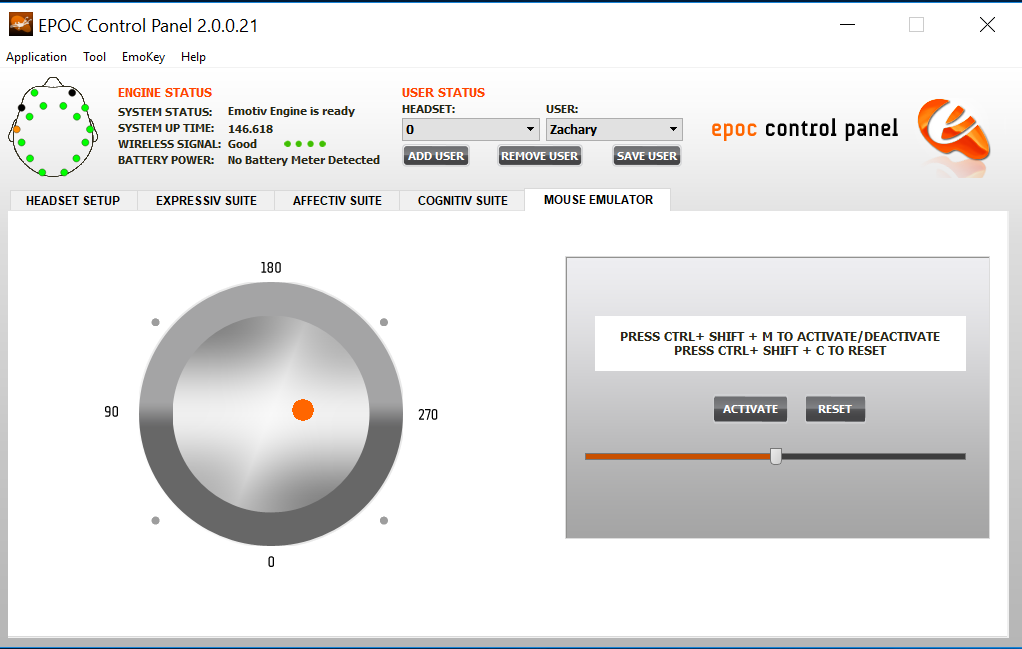
\includegraphics[scale=0.4]{mouse.png}\\
 				\end{center}

		\subsection{Demonstrate its Ability to Read EEG Signals}
			\paragraph{}
				Now that the headset is connected and all the electrodes have a good signal I started to record my EEG signal over time.  In the below graph of my EEG you can see that in 
				the first few measurements my eyes were closed and i tried to think as little as 
				possible and my signal is the lowest even thouching the line deamed meditation.  In 
				middle of the measurement i started doing a speed math test with simple mental math 
				questions with a time limit and you can see my signal and excitment increases, before 
				i finally relax again for the last measurements in the EEG.  In retrospect I wish i 
				found something more excitable for my brain as the mental math had a smaller expect 
				then i anticpated.

				\begin{center}
					\includegraphics[scale=0.4]{EEG.png}\\
 				\end{center}
	
	\section{Task B: Read Your EOG Signal with Epoc Emotive}
		\paragraph{}
			To demostrate the ability of the headset to measure and read our EOG signals we used the 
			expressive suite in the program. I found that after practicing for a while adjusting the 
			sensativity would only make the readins worse except for blink.  The robot was able to 
			emulate the blinking, winking, smiling, and etc. These actions could then be mapped to 
			certain keys on the keyboard to type or later control and play Mario Kart. I assigned 
			blink to "Z", wink to "A", smile to "C", and raise eyebrows to "H" and then in opening 
			notepad after some practice i was able to correctly type my name.  Below is an included 
			picture to show as many emotions as possible. I smiled, raised my eyebrows, and blinked.
			Unfortuntely i missed the blink in the snapshot but the rest can be seen.

			\begin{center}
				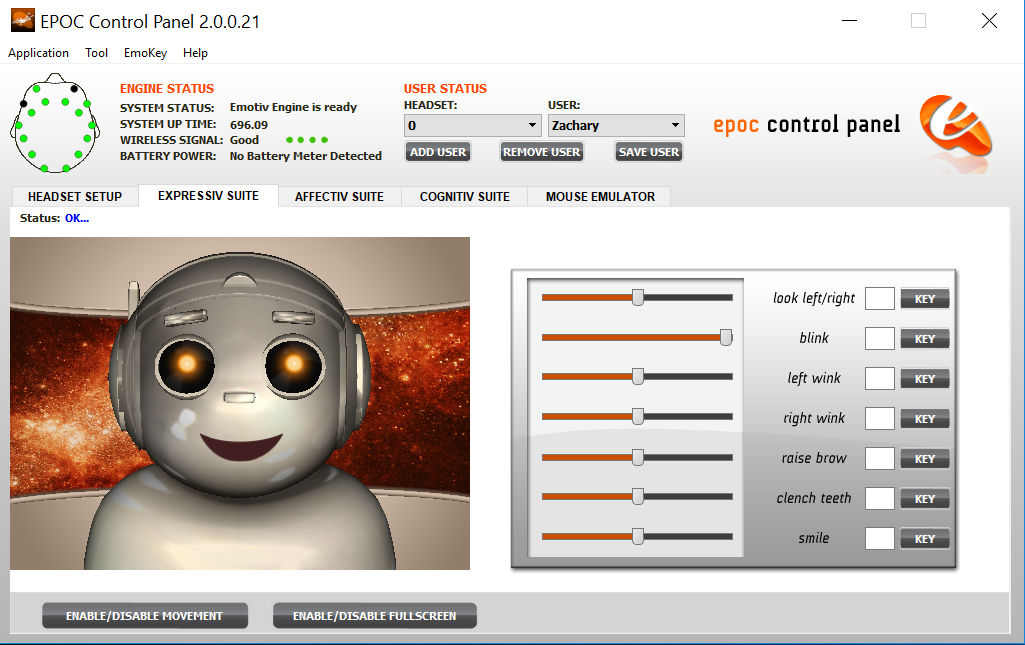
\includegraphics[scale=0.5]{express.png}\\
 			\end{center}

 	\section{Task C: Use the Headset to Complete Laps in Mario Kart}
 		\subsection{Training My Brain}
 			\paragraph{}
 				The next task is to control a car in Mario Kart around a couple laps using my brain 
 				to trigger certain keystrokes.  To do this unlike some of my classmates i choose to 
 				use the cognitiv suite rather than the expressive suite because i felt like i could 
 				have better control.  I spent a good amount of time trying to train myself.  My goal 
 				was to train my brain to PUSH, LEFT and, RIGHT control the box.  After struggling 
 				for a while i researched some of emotives resources for help in the hopes to have 
 				better success.  Their first suggestion was to read something simple while training 
 				your nuetral state.  This helped a lot because to have real control you need to not 
 				only be able to start moving the box, but also stop it and if you did as i did at 
 				first and keep your eyes closed you will never realisticlly be able to stop moving 
 				the box in practice.  Also it suggested watching objects in real life or on youtube 
 				while training to help maintain focus on the task your are trying to perform.  Their 
 				final suggestion was essentially time and practice it is easy for you to exhaust your
 				brain in training which will hurt the signal integrety so i would periodically stop 
 				training and read or watch tv to relax my brain.  Below you can see me pushing the 
 				box as well as moving it to the left.

 				\begin{center}
					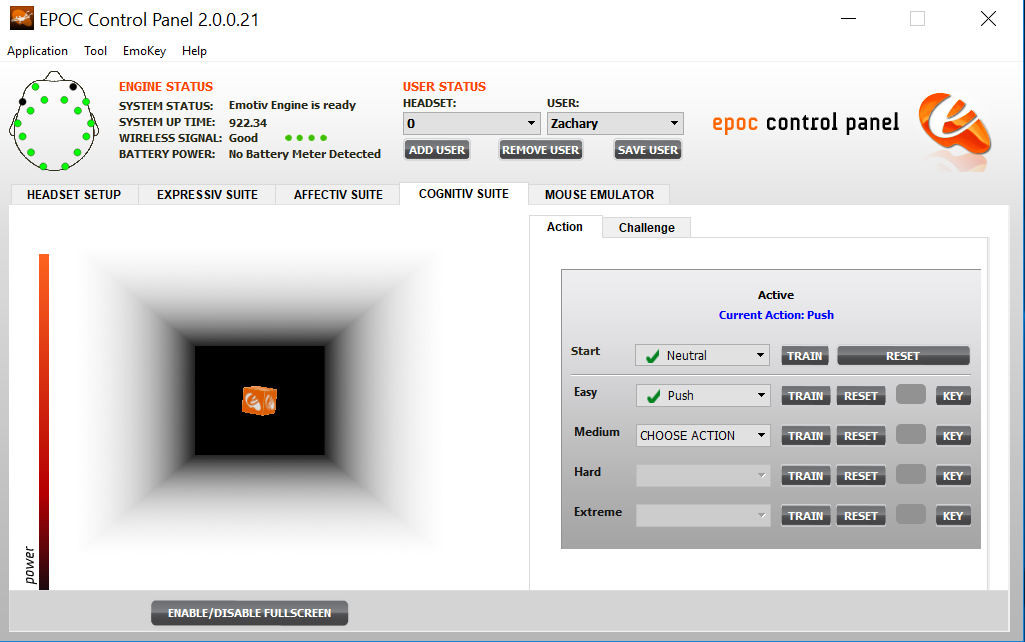
\includegraphics[scale=0.4]{push.png}\\
					\vspace{2mm}
					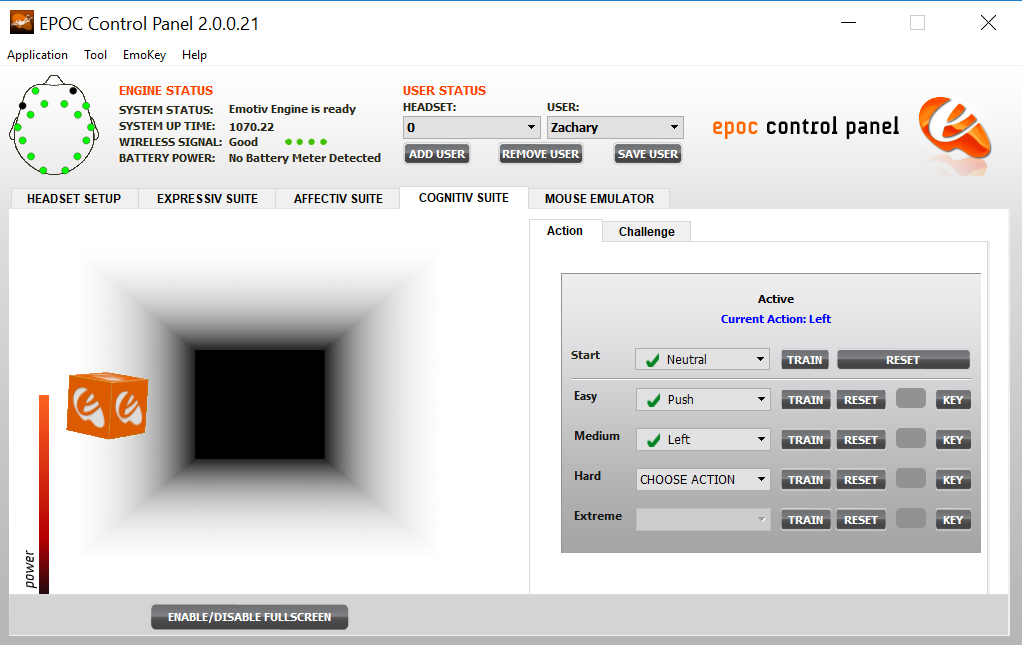
\includegraphics[scale=0.4]{left.png}\\
 				\end{center}

 				To translate this to racing in Mario Kart I mapped push to holding the "W" key, left 
 				to holding the "A" key, and right to the "D" key, which i then mapped to forward, 
 				left, and right respectively to drive the car.  Thankfully in Mario Kart you do not 
 				need to brake ever.  Below I have included a link to my video of me doing three hot 
 				laps of a Mario Kart track.  It is worth mentioning you can see that it takes me a 
 				while to start having control of the car in the beginning of the first lap and the second lap is easily my best. But by the end of the second lap and into the third 
 				lap you can see that my brain was getting tired and failure to do what i wanted 
 				propagated into larger and larger errors.  My camera setup is sub par but you are 
 				able to see me the game and keyboard.  To insure that i am not using the
 				conventional keyboard i keep my hands below the table.  Below are my lap times.

 				\begin{center}
					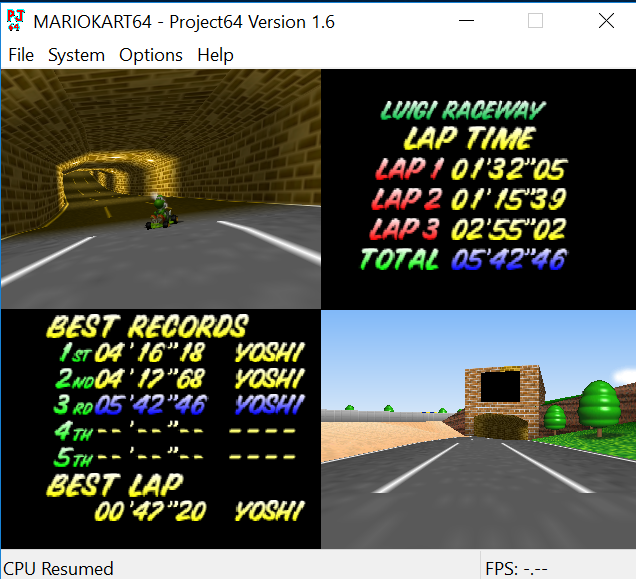
\includegraphics[scale=0.7]{mario.png}\\
					\href{https://drive.google.com/open?id=1dnGApt-1-puP1PLlY33D6uRe2Z6nUfDU}
					{Time Trial Video}
 				\end{center}
\end{document}
%%%%%%%%%%